\documentclass{../../slides-style}

\slidetitle[Высокий уровень]{Работа с сетью}{12.10.2022}

\begin{document}

    \begin{frame}[plain]
        \titlepage
    \end{frame}

    \section{Теоретическое введение}

    \begin{frame}
        \frametitle{Протоколы прикладного уровня}
        \begin{itemize}
            \item Если вы пользуетесь ``голыми'' сокетами под .NET, скорее всего, вы делаете что-то не так
            \item TCP и UDP обеспечивают транспорт, вся полезная работа делается протоколами прикладного уровня
            \item Их тысячи:
            \begin{itemize}
                \item DNS
                \item Электронная почта: SMTP, IMAP, POP3
                \item Различные виды удалённого вызова: WCF, Apache Thrift, gRPC, ...
                \item WWW: HTTP, HTTPS
                \item Стриминг: RTP, RTCP
                \item P2P и доставка контента: BitTorrent
                \item ...
            \end{itemize}
        \end{itemize}
    \end{frame}

    \begin{frame}
        \frametitle{Как работает браузер}
        \begin{enumerate}
            \item Определяет URL, указывающий на желаемую страницу
            \item Выполняет DNS-запрос на доменное имя из URL, узнаёт IP
            \item Устанавливает TCP-соединение с портом 80 целевой машины
            \item Отправляет HTTP-запрос на получение файла
            \item Получает ответ от сервера с HTML-страницей
            \item Если страница содержит URL, необходимые для её отображения, браузер повторяет процесс
            \begin{itemize}
                \item Картинки, скрипты, стили и т.д.
            \end{itemize}
            \item Браузер отображает страницу, отдаёт скрипты на интерпретацию, при необходимости запускает плагины
            \item Если новых запросов некоторое время не поступает, браузер разрывает соединение с сервером
        \end{enumerate}
    \end{frame}

    \begin{frame}[fragile]
        \frametitle{Протокол HTTP}
        \begin{itemize}
            \item Простой текстовый протокол поверх TCP
            \item Запрос-ответ
            \item Вид запроса:
            \begin{minted}{text}
<Метод> параметр <версия протокола>
<Заголовки>
<Тело запроса>
<Пустая строка>
            \end{minted}
        \end{itemize}
    \end{frame}

    \begin{frame}[fragile]
        \frametitle{Пример}
        \framesubtitle{Слегка сокращённый}
        \begin{minted}{text}
GET http://se.math.spbu.ru/SE HTTP/1.1
Host: se.math.spbu.ru
Connection: keep-alive
Upgrade-Insecure-Requests: 1
User-Agent: Chrome/68.0.3440.106 
Accept: text/html,application/xhtml+xml
Referer: http://se.math.spbu.ru/
Accept-Encoding: gzip, deflate
Accept-Language: ru-RU,ru;q=0.9,en-US;q=0.8,en;q=0.7

        \end{minted}
    \end{frame}

    \begin{frame}[fragile]
        \frametitle{Ответ}
        \framesubtitle{Очень сокращённый}
        \begin{small}
            \begin{minted}{text}
HTTP/1.1 200 OK
Server: Zope/(Zope 2.10.6-final, python 2.4.6, linux2) ZServer/1.1 Plone/3.1.3
Date: Sat, 01 Sep 2018 12:57:32 GMT
Content-Length: 29068
Content-Language: ru
Expires: Sat, 1 Jan 2000 00:00:00 GMT
Content-Type: text/html;charset=utf-8

<!DOCTYPE html ...>
<html xmlns="http://www.w3.org/1999/xhtml" xml:lang="ru"
      lang="ru">
  <head>
  </head>
  <body>
  </body>
</html>
            \end{minted}
        \end{small}
    \end{frame}

    \begin{frame}
        \frametitle{Виды запросов}
        \framesubtitle{Методы}
        \begin{itemize}
            \item \textbf{GET} --- получить страницу
            \item \textbf{HEAD} --- получить только заголовок
            \item \textbf{PUT} --- залить новую страницу на сервер
            \item \textbf{POST} --- добавить что-нибудь к странице
            \item \textbf{DELETE} --- удалить страницу
            \item \textbf{TRACE} --- отправить запрос обратно (для отладки)
            \item \textbf{CONNECT} --- подключиться через прокси
            \item \textbf{OPTIONS} --- узнать, что можно использовать
        \end{itemize}
    \end{frame}

    \begin{frame}
        \frametitle{Коды ответов}
        \begin{small}
            \begin{tabu} {| X[0.3 l p] | X[0.5 l p] | X[1 l p] |}
                \tabucline-
                Код  & Значение         & Примеры                                                       \\
                \tabucline-
                \everyrow{\tabucline-}
                1xx  & Информация       & 100 --- сервер согласен обрабатывать запросы                  \\
                2xx  & Успех            & 200 --- запрос успешно обработан, 204 --- ответ пустой        \\
                3xx  & Перенаправление  & 301 --- страница перемещена, 304 --- возьмите из своего кэша  \\
                4xx  & Ошибка клиента   & 404 --- страница не найдена, 403 --- нет прав                 \\
                5xx  & Ошибка сервера   & 500 --- сервер упал, 503 --- попробуйте позже                 \\
            \end{tabu}
        \end{small}
    \end{frame}

    \section{Как это работает в .NET}

    \begin{frame}[fragile]
        \frametitle{Как это работает в .NET}
        \framesubtitle{HttpClient}
        \begin{minted}{csharp}
class Program
{
    private static async Task Main(string[] args)
    {
        var httpClient = new HttpClient();

        var response = await httpClient.GetAsync("http://hwproj.me/");
        if (response.IsSuccessStatusCode)
        {
            var content = await response.Content.ReadAsStringAsync();
            Console.WriteLine(content);
        }
    }
}
        \end{minted}
    \end{frame}

    \begin{frame}[fragile]
        \frametitle{Exponential backoff}
        \begin{footnotesize}
            \begin{minted}{csharp}
static async Task<string> DownloadStringWithRetries(string uri)
{
    using (var client = new HttpClient()) {
        var delay = TimeSpan.FromSeconds(1);
        for (int i = 0; i != 3; ++i) {
            try {
                return await client.GetStringAsync(uri);
            } catch {
            }
            await Task.Delay(delay);
            delay *= 2;
        }

        // Попробуем последний раз, дав ошибке распространиться
        return await client.GetStringAsync(uri);
    }
}
            \end{minted}
        \end{footnotesize}
    \end{frame}

    \section{Веб-сервисы}

    \begin{frame}
        \frametitle{Зачем всё это?}
        \begin{itemize}
            \item Писать свой браузер можно, но не нужно
            \item HTTP --- основа для протоколов общения ``приложение-приложение''
            \item Веб-сервисы --- страницы в интернете, предназначенные не для браузеров, а для других приложений
            \begin{itemize}
                \item Интерфейс для облачных сервисов типа GMail, Google Drive, ВКонтакте, Twitter и т.д.
                \begin{itemize}
                    \item Браузерные клиенты часто пользуются тем же API, что доступен сторонним разработчикам
                \end{itemize}
                \item Публичные API для приложений (например, бэкапы смартфонов)
                \item Распределённые приложения в одной корпоративной сети
                \begin{itemize}
                    \item Сервер базы данных, сервер бизнес-логики, сервера вспомогательных служб со своими API
                \end{itemize}
            \end{itemize}
        \end{itemize}
    \end{frame}

    \begin{frame}
        \frametitle{Как оно работает}
        \begin{itemize}
            \item Удалённый вызов --- клиент посылает HTTP-запрос с именем метода и параметрами, сервер исполняет запрос и отправляет ответ обратно
            \item Требуется сериализация: XML, JSON, protobuf, ...
            \item Требуется механизм общения сервера и клиента:
            \begin{itemize}
                \item SOAP --- старый, громоздкий, но до сих пор очень популярный протокол, использует XML
                \item WCF --- библиотека для разработки веб-сервисов под .NET, несколько устарела, но до сих пор очень популярна, может использовать SOAP
                \item REST --- легковесный протокол общения, очень-очень популярен
            \end{itemize}
            \item Машиночитаемое описание возможностей веб-сервиса
        \end{itemize}
    \end{frame}

    \section{REST}

    \begin{frame}
        \frametitle{Representational State Transfer}
        \framesubtitle{REST}
        \begin{itemize}
            \item ``Легковесный'' интерфейс для веб-сервисов, построенный на HTTP-запросах
            \item Запрос и его параметры передаются в основном через URL
            \begin{itemize}
                \item Иногда используется тело HTTP-запроса с JSON или бинарными данными
            \end{itemize}
            \item Сервер не хранит состояние сессии, запросы всё таскают с собой
            \begin{itemize}
                \item Удобно, запрос может прийти откуда угодно и когда угодно, лишь бы он был правильный
            \end{itemize}
        \end{itemize}
    \end{frame}

    \begin{frame}
        \frametitle{Интерфейс сервиса}
        \begin{itemize}
            \item Коллекции
            \begin{itemize}
                \item http://api.example.com/resources/
            \end{itemize}
            \item Элементы
            \begin{itemize}
                \item http://api.example.com/resources/item/17
            \end{itemize}
            \item HTTP-методы
            \begin{itemize}
                \item GET
                \item PUT
                \item POST
                \item DELETE
            \end{itemize}
            \item Передача параметров прямо в URL
            \begin{itemize}
                \item http://api.example.com/resources?user=me\&access\_token=ASFQF
            \end{itemize}
        \end{itemize}
    \end{frame}

    \begin{frame}
        \frametitle{Пример, Google Drive REST API}
        \begin{itemize}
            \item GET \url{https://www.googleapis.com/drive/v2/files} --- список всех файлов
            \item GET \url{https://www.googleapis.com/drive/v2/files/fileId} --- метаданные файла по его Id
            \item POST \url{https://www.googleapis.com/upload/drive/v2/files} — загрузить новый файл
            \item PUT \url{https://www.googleapis.com/upload/drive/v2/files/fileId} --- обновить файл
            \item DELETE \url{https://www.googleapis.com/drive/v2/files/fileId} --- удалить файл
        \end{itemize}
    \end{frame}

    \begin{frame}[fragile]
        \frametitle{REST и HttpClient}
        \framesubtitle{Сырой REST}
        \begin{footnotesize}
            \begin{minted}{csharp}
private static async Task Main(string[] args)
{
    var httpClient = new System.Net.Http.HttpClient();

    var request = "https://api.exchangeratesapi.io/latest?base=USD&symbols=RUB";
    var response = await httpClient.GetAsync(request);
    if (response.IsSuccessStatusCode)
    {
        var content = await response.Content.ReadAsStringAsync();
        var data = JsonConvert.DeserializeObject<JObject>(content);
        var baseCurrency = data["base"];
        var ruble = data.Value<JToken>("rates").Values<JProperty>().First();
        Console.WriteLine($"1 {baseCurrency} = {ruble.Value} {ruble.Name}");
    }
}
            \end{minted}
        \end{footnotesize}
    \end{frame}

    \begin{frame}[fragile]
        \frametitle{REST и клиентские библиотеки}
        \framesubtitle{Google Drive API}
        \begin{scriptsize}
            \begin{minted}{csharp}
class Program
{
    private static readonly string[] Scopes = { DriveService.Scope.DriveReadonly };
    private const string ApplicationName = "GDriveDemo";

    static async Task Main(string[] args) {
        UserCredential credential;

        using (var stream =
            new FileStream("credentials.json", FileMode.Open, FileAccess.Read)) {
            var credPath = "token.json";
            credential = await GoogleWebAuthorizationBroker.AuthorizeAsync(
                GoogleClientSecrets.Load(stream).Secrets,
                Scopes,
                "user",
                CancellationToken.None,
                new FileDataStore(credPath, true));
            Console.WriteLine("Credential file saved to: " + credPath);
        }
        ...
    }
}
            \end{minted}
        \end{scriptsize}
    \end{frame}

    \begin{frame}[fragile]
        \frametitle{Google Drive API (2)}
        \begin{scriptsize}
            \begin{minted}{csharp}
class Program
{
    ...
    static async Task Main(string[] args) {
        UserCredential credential;
        ...
        var service = new DriveService(new BaseClientService.Initializer() {
            HttpClientInitializer = credential,
            ApplicationName = ApplicationName,
        });

        FilesResource.ListRequest listRequest = service.Files.List();
        listRequest.PageSize = 10;
        listRequest.Fields = "nextPageToken, files(id, name)";
        ...
    }
}
            \end{minted}
        \end{scriptsize}
    \end{frame}

    \begin{frame}[fragile]
        \frametitle{Google Drive API (3)}
        \begin{scriptsize}
            \begin{minted}{csharp}
class Program
{
    ....
    static async Task Main(string[] args) {
        FilesResource.ListRequest listRequest = service.Files.List();
        ...
        IList<Google.Apis.Drive.v3.Data.File> files = listRequest.Execute().Files;
        Console.WriteLine("Files:");
        if (files != null && files.Count > 0) {
            foreach (var file in files) {
                Console.WriteLine($"{file.Name} ({file.Id})");
            }
        } else {
            Console.WriteLine("No files found.");
        }
        Console.Read();
    }
}
            \end{minted}
        \end{scriptsize}
    \end{frame}

    \section{Отладка веб-сервисов}

    \begin{frame}
        \frametitle{Как это отлаживать}
        \framesubtitle{Fiddler}
        \begin{center}
            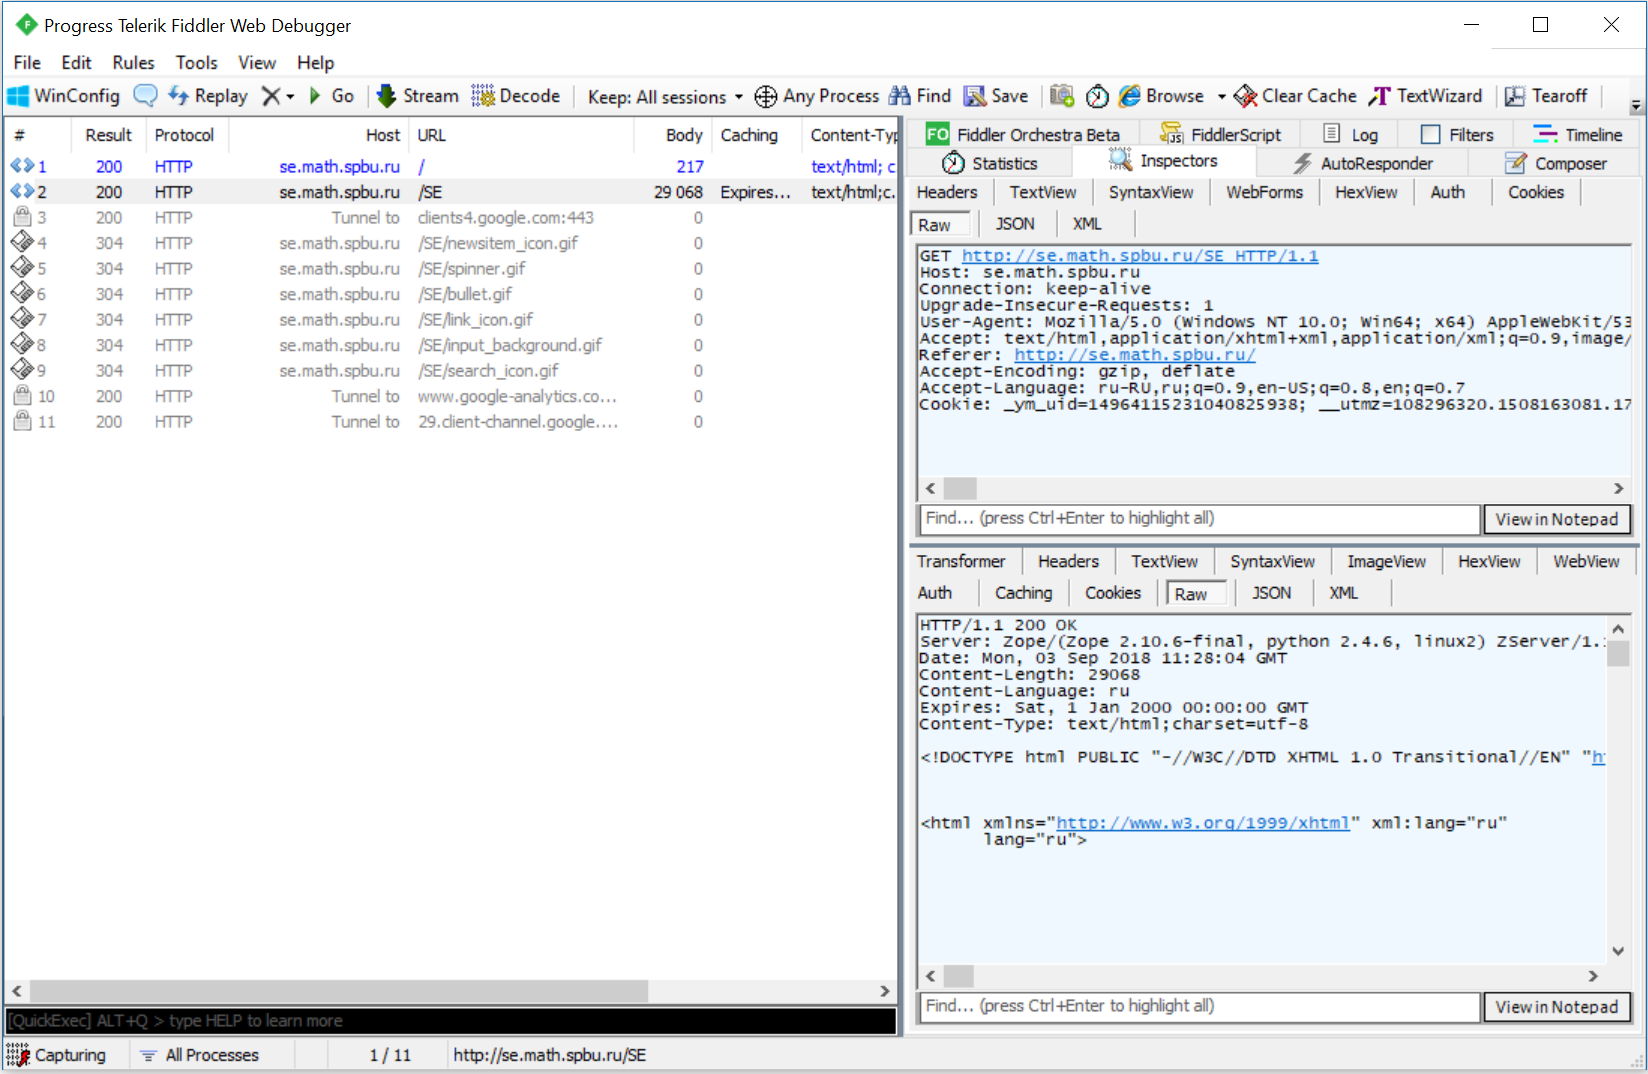
\includegraphics[width=0.9\textwidth]{fiddler.png}
        \end{center}
    \end{frame}

    \section{Безопасность}

    \begin{frame}
        \frametitle{Сетевая безопасность}
        \begin{itemize}
            \item Почти все сервисы требуют авторизации и обеспечения безопасности
            \item Аутентификация --- установление личности (точнее, идентичности) участника взаимодействия
            \begin{itemize}
                \item Обычно взаимна
            \end{itemize}
            \item Авторизация --- установление прав на выполнение операции
            \item Шифрование --- обеспечение конфиденциальности передаваемой информации
            \item Также важны:
            \begin{itemize}
                \item Целостность --- злоумышлениик ничего не поменял
                \item Актуальность --- злоумышленник не проиграл старое сообщение
            \end{itemize} 
        \end{itemize}
    \end{frame}

    \begin{frame}
        \frametitle{Шифрование}
        \begin{center}
            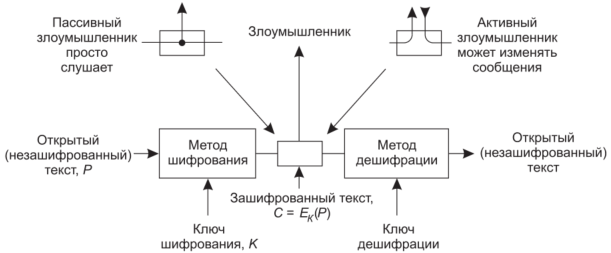
\includegraphics[width=0.6\textwidth]{cryptography.png}
            \attribution{Э. Таненбаум}
        \end{center}
        \begin{itemize}
            \item Алгоритм шифрования считается известным, секретен только ключ
            \item Усложнение алгоритма шифрования не всегда повышает криптостойкость
        \end{itemize}
        \begin{textblock}{2.5}(0,-10)
            
\includegraphics[width=\textwidth]{youAreBeingWatched.png}
        \end{textblock}
    \end{frame}

    \begin{frame}
        \frametitle{Шифрование с открытым ключом}
        \begin{itemize}
            \item Алгоритм делится на две части, D и E, так, что D(E(P)) = P
            \item D очень сложно получить по E
            \begin{itemize}
                \item Например, найти простые сомножители огромного числа или дискретный логарифм по заданному модулю
            \end{itemize}
            \item D (ключ от D) держится в секрете, E выкладывается в открытый доступ
            \item Если Боб хочет послать Алисе сообщение, он берёт её открытый ключ $E_A$, шифрует им сообщение $P$ и отправляет Алисе
            \item Алиса дешифрует сообщение, вычисляя $D_A(E_A(P))$
            \item У каждого пользователя своя пара ключей
            \item Алгоритмы: RSA, ElGamal, эллиптические шифры
        \end{itemize}
    \end{frame}

    \begin{frame}
        \frametitle{Цифровые подписи}
        \begin{center}
            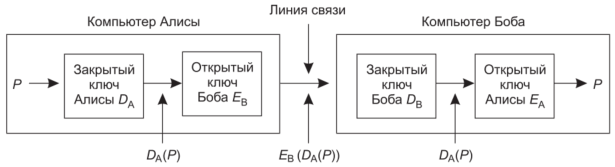
\includegraphics[width=0.7\textwidth]{signature.png}
            \attribution{Э. Таненбаум}
        \end{center}
        \begin{itemize}
            \item Надо, чтобы $D(E(P)) = P$ (это так для большинства криптосхем)
            \item Шифровать всё сообщение слишком медленно
            \item Message Digest-ы --- хорошие хеши сообщений
            \begin{itemize}
                \item MD5, SHA-1, SHA-2, SHA-3
                \item MD5 уязвим, SHA-1 уязвим чуть менее
            \end{itemize}
            \item Подписывается только хеш, это почти так же криптостойко, но в сотни раз быстрее
        \end{itemize}
    \end{frame}

    \begin{frame}
        \frametitle{Сертификаты}
        \begin{center}
            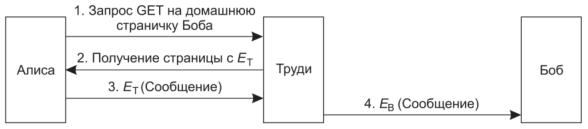
\includegraphics[width=0.6\textwidth]{manInTheMiddle.png}
            \attribution{Э. Таненбаум}
        \end{center}
        \begin{itemize}
            \item Сертификат --- сообщение, подтверждающее идентичность ключа, подписанное Certificate Authority (стандарт X.509)
            \item Цепочка сертификатов --- CA верхнего уровня подписывает сертификаты CA уровнем ниже, чтобы они могли подписывать сертификаты пользователей
            \item Корневые сертификаты --- сертификаты, которым принято доверять
            \item Самоподписанные сертификаты --- не доверенные, используются для отладки
        \end{itemize}
    \end{frame}

    \begin{frame}
        \frametitle{HTTPS}
        \begin{center}
            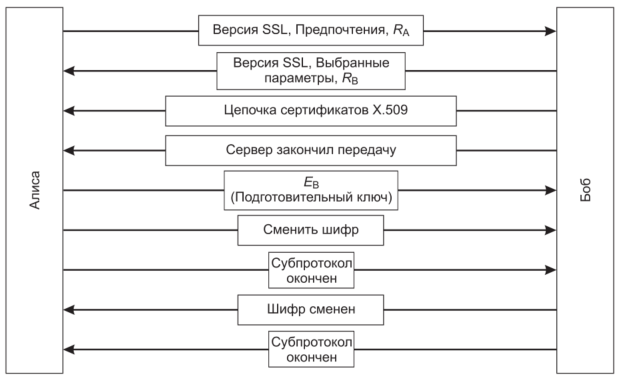
\includegraphics[width=0.6\textwidth]{ssl.png}
            \attribution{Э. Таненбаум}
        \end{center}
        \begin{itemize}
            \item SSL (Secure Sockets Layer)
            \item HTTPS --- HTTP через SSL
        \end{itemize}
    \end{frame}

    \begin{frame}
        \frametitle{OAuth 2}
        \begin{center}
            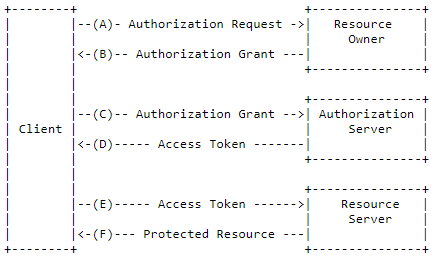
\includegraphics[width=0.5\textwidth]{oauth.png}
            \attribution{RFC 6749}
        \end{center}
        \begin{itemize}
            \item Позволяет разрешить пользование ресурсом, не раскрывая хозяину ресурса логин и пароль пользователя
            \begin{itemize}
                \item Логин по аккаунту в Google или аккаунту в VK
            \end{itemize}
        \end{itemize}
    \end{frame}

\end{document}
